\renewcommand*{\arraystretch}{1.1}

\noindent\begin{tabularx}{17cm}{|>{\small \sf}c|X|}
	\hline
	query    & BI / 10 \\ \hline
%
	title       & Central Person for a Tag \\ \hline
%
    pattern     & \hfill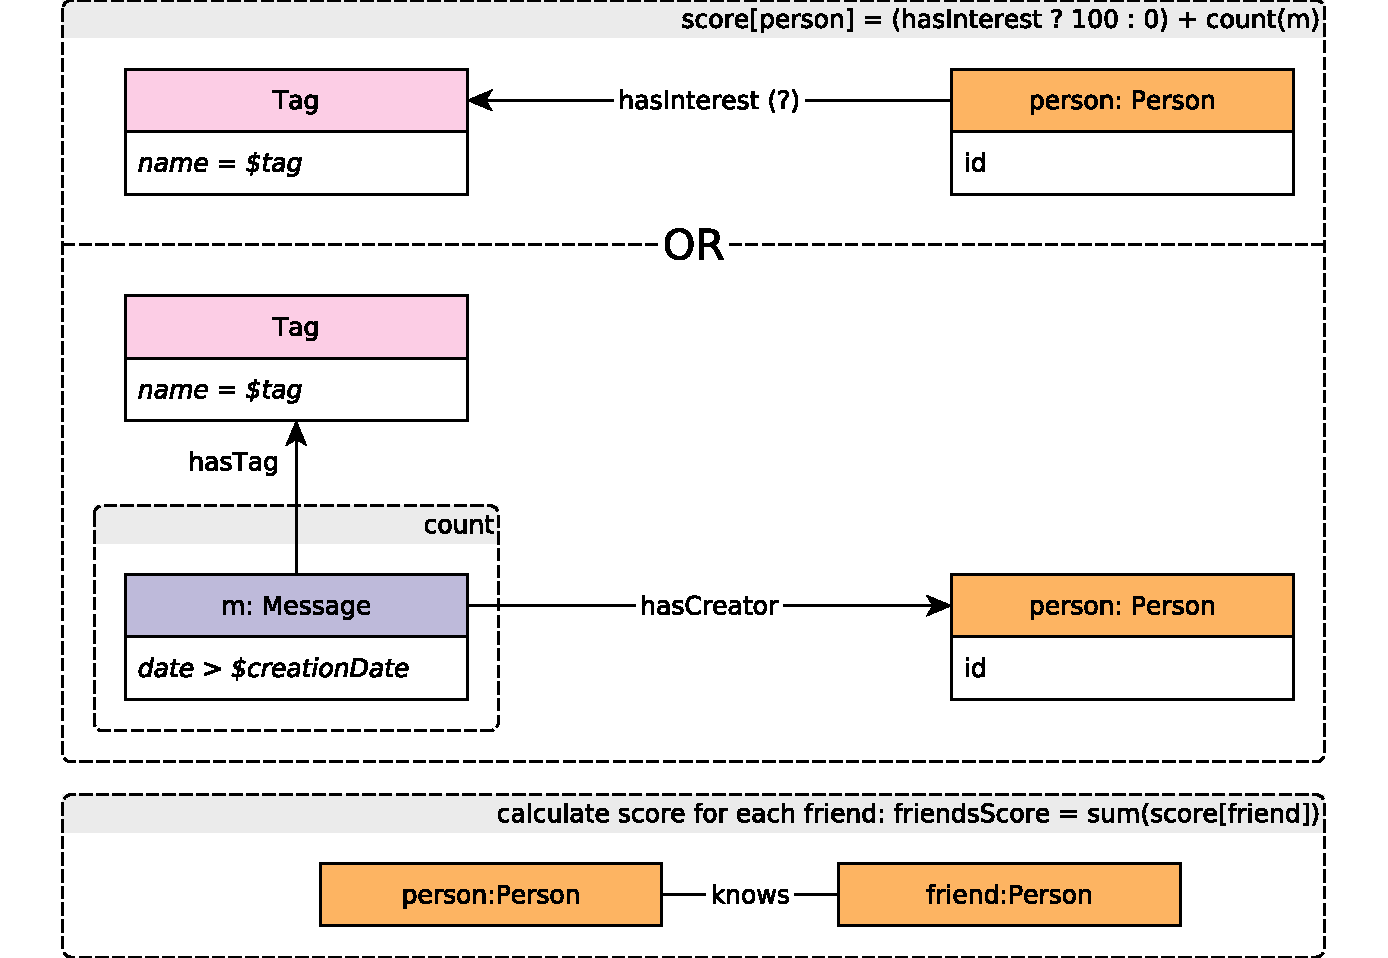
\includegraphics[scale=\patternscale,margin=0cm .2cm]{patterns/bi-read-10}\hfill\vadjust{} \\ \hline
%
	desc. & Given a Tag, find all Persons that are either interested in the Tag, or
have written a Message (Post or Comment) with creation date after a
given date and that has a given Tag. For each Person, compute the score
as the sum of the following two aspects:

\begin{itemize}
\tightlist
\item
  100, if the Person has this tag as their interest, or 0 otherwise
\item
  number of messages by this person with the given tag
\end{itemize}
 \\ \hline
%
	
%
	params  &
	\vspace{1.1ex}{\begin{tabularx}{14.66cm}{|c|M|m{2cm}|Y|} \hline
	\cellcolor{parameter} \color{white} \footnotesize $\mathsf{1}$ & \varname{tag} & \cellcolor{gray!20} \vartype{32-bit Integer} &  \\ \hline
	\cellcolor{parameter} \color{white} \footnotesize $\mathsf{2}$ & \varname{date} & \cellcolor{gray!20} \vartype{Date} &  \\ \hline
	\end{tabularx}}\vspace{1.1ex} \\ \hline
%
	
	result      &
	\vspace{1.1ex}{\begin{tabularx}{14.66cm}{|c|M|m{2cm}|c|Y|} \hline
	\cellcolor{result} \color{white} \footnotesize $\mathsf{1}$ & \varname{person.id} & \cellcolor{gray!20} \vartype{64-bit Integer} &
	    \texttt{R} &
	     \\ \hline
	\cellcolor{result} \color{white} \footnotesize $\mathsf{2}$ & \varname{score} & \cellcolor{gray!20} \vartype{32-bit Integer} &
	    \texttt{A} &
	     \\ \hline
	\cellcolor{result} \color{white} \footnotesize $\mathsf{3}$ & \varname{friendsScore} & \cellcolor{gray!20} \vartype{32-bit Integer} &
	    \texttt{A} &
	    The sum of the score of the Person's friends \\ \hline
	\end{tabularx}}\vspace{1.1ex} \\ \hline
	
%
	sort        &
	\vspace{1.1ex}{\begin{tabular}{|c|l|c|} \hline
	\cellcolor{sort} \color{white} \footnotesize $\mathsf{1}$ & \varname{score + friendsScore} & \cellcolor{gray!20} $\desc$ \\ \hline
	\cellcolor{sort} \color{white} \footnotesize $\mathsf{2}$ & \varname{person.id} & \cellcolor{gray!20} $\asc$ \\ \hline
	\end{tabular}}\vspace{1.1ex} \\ \hline
	%
	limit       & 100 \\ \hline
	%
	CPs &
	\multicolumn{1}{>{\raggedright}l|}{
	  \chokepoint{1.2}, 
	  \chokepoint{2.1}, 
	  \chokepoint{2.3}, 
	  \chokepoint{3.2}
	  } \\ \hline
	%
    %
\end{tabularx}
\vspace{2ex}